\documentclass[12pt]{article}

\usepackage{fullpage}
\usepackage{multicol,multirow}
\usepackage{tabularx}
\usepackage{listings}
\usepackage[utf8]{inputenc}
\usepackage[russian]{babel}
\usepackage{graphicx}
\usepackage{csquotes}

\begin{document}

\begin{titlepage}

    \begin{center}

        \bfseries
        {\small Московский авиационный институт\\ 
        (национальный исследовательский университет)}

        % \vspace{48pt}
        {\small Факультет информационных технологий и прикладной 
        математики}
        
        % \vspace{36pt}
        {\small Кафедра вычислительной математики и программирования}
        
        \vspace{8cm}
        {\Large Лабораторная работа \textnumero 2 по курсу} 
        \enquote{\Large Компьютерная графика}
        
    \end{center}
    
    \vspace{84pt}
    \begin{flushright}
        \begin{tabular}{rl}
            Студент: & Е.Ю. Юрков \\
            % Преподаватель: &  \\
            Группа: & М80-312Б-22 \\
            Дата: & \\
            Оценка: & \\
            Подпись: & \\
        \end{tabular}
    \end{flushright}
    
    \vfill
    
    \begin{center}
        
        \bfseries
        Москва, \the\year
    
    \end{center}

\end{titlepage}

% Выполнил студент группы М8О-312Б-22 МАИ \textit{Юрков Евгений}.

\subsection*{Цель лабораторной работы}

В этой лабораторной работе вы познакомитесь с основами 3D-графики: построением
простых 3D-объектов, проекцией на 2D-плоскость, а также научитесь работать с матрицами
перспективы и ортографической проекции.

\subsection*{Задача}

\textbf{Вариант 7. Построение 3D-сцены с несколькими объектами}

Постройте сцену, содержащую куб, пирамиду и сферу.
Используйте перспективную проекцию для отображения сцены.
Реализуйте возможность перемещения камеры по сцене с помощью клавиатуры.
Дополнительно: Реализуйте возможность приближения и удаления камеры от объектов с
плавным изменением угла обзора.

% \newpage
\subsection*{Метод решения}

Для выполнения поставленной задачи было принято решение использовать
язык программирования C++ и библиотеки SFML и OpenGL.
Также использовалась библиотека glm для операций с векторами и матрицами.
Была создана сцена с кубом, сферой и пирамидой.
Камеру можно было переключать между этими объектами и вращать вокруг них.

Для построения фигур были реализованы классы Shape, Sphere, Cube, Pyramid.
А для камеры был реализован класс Camera

Также на каждой итерации цикла вычисляется коэффициент растяжения фигуры,
для изменения её формы (дополнительное задание).

\subsection*{Результат работы программы}

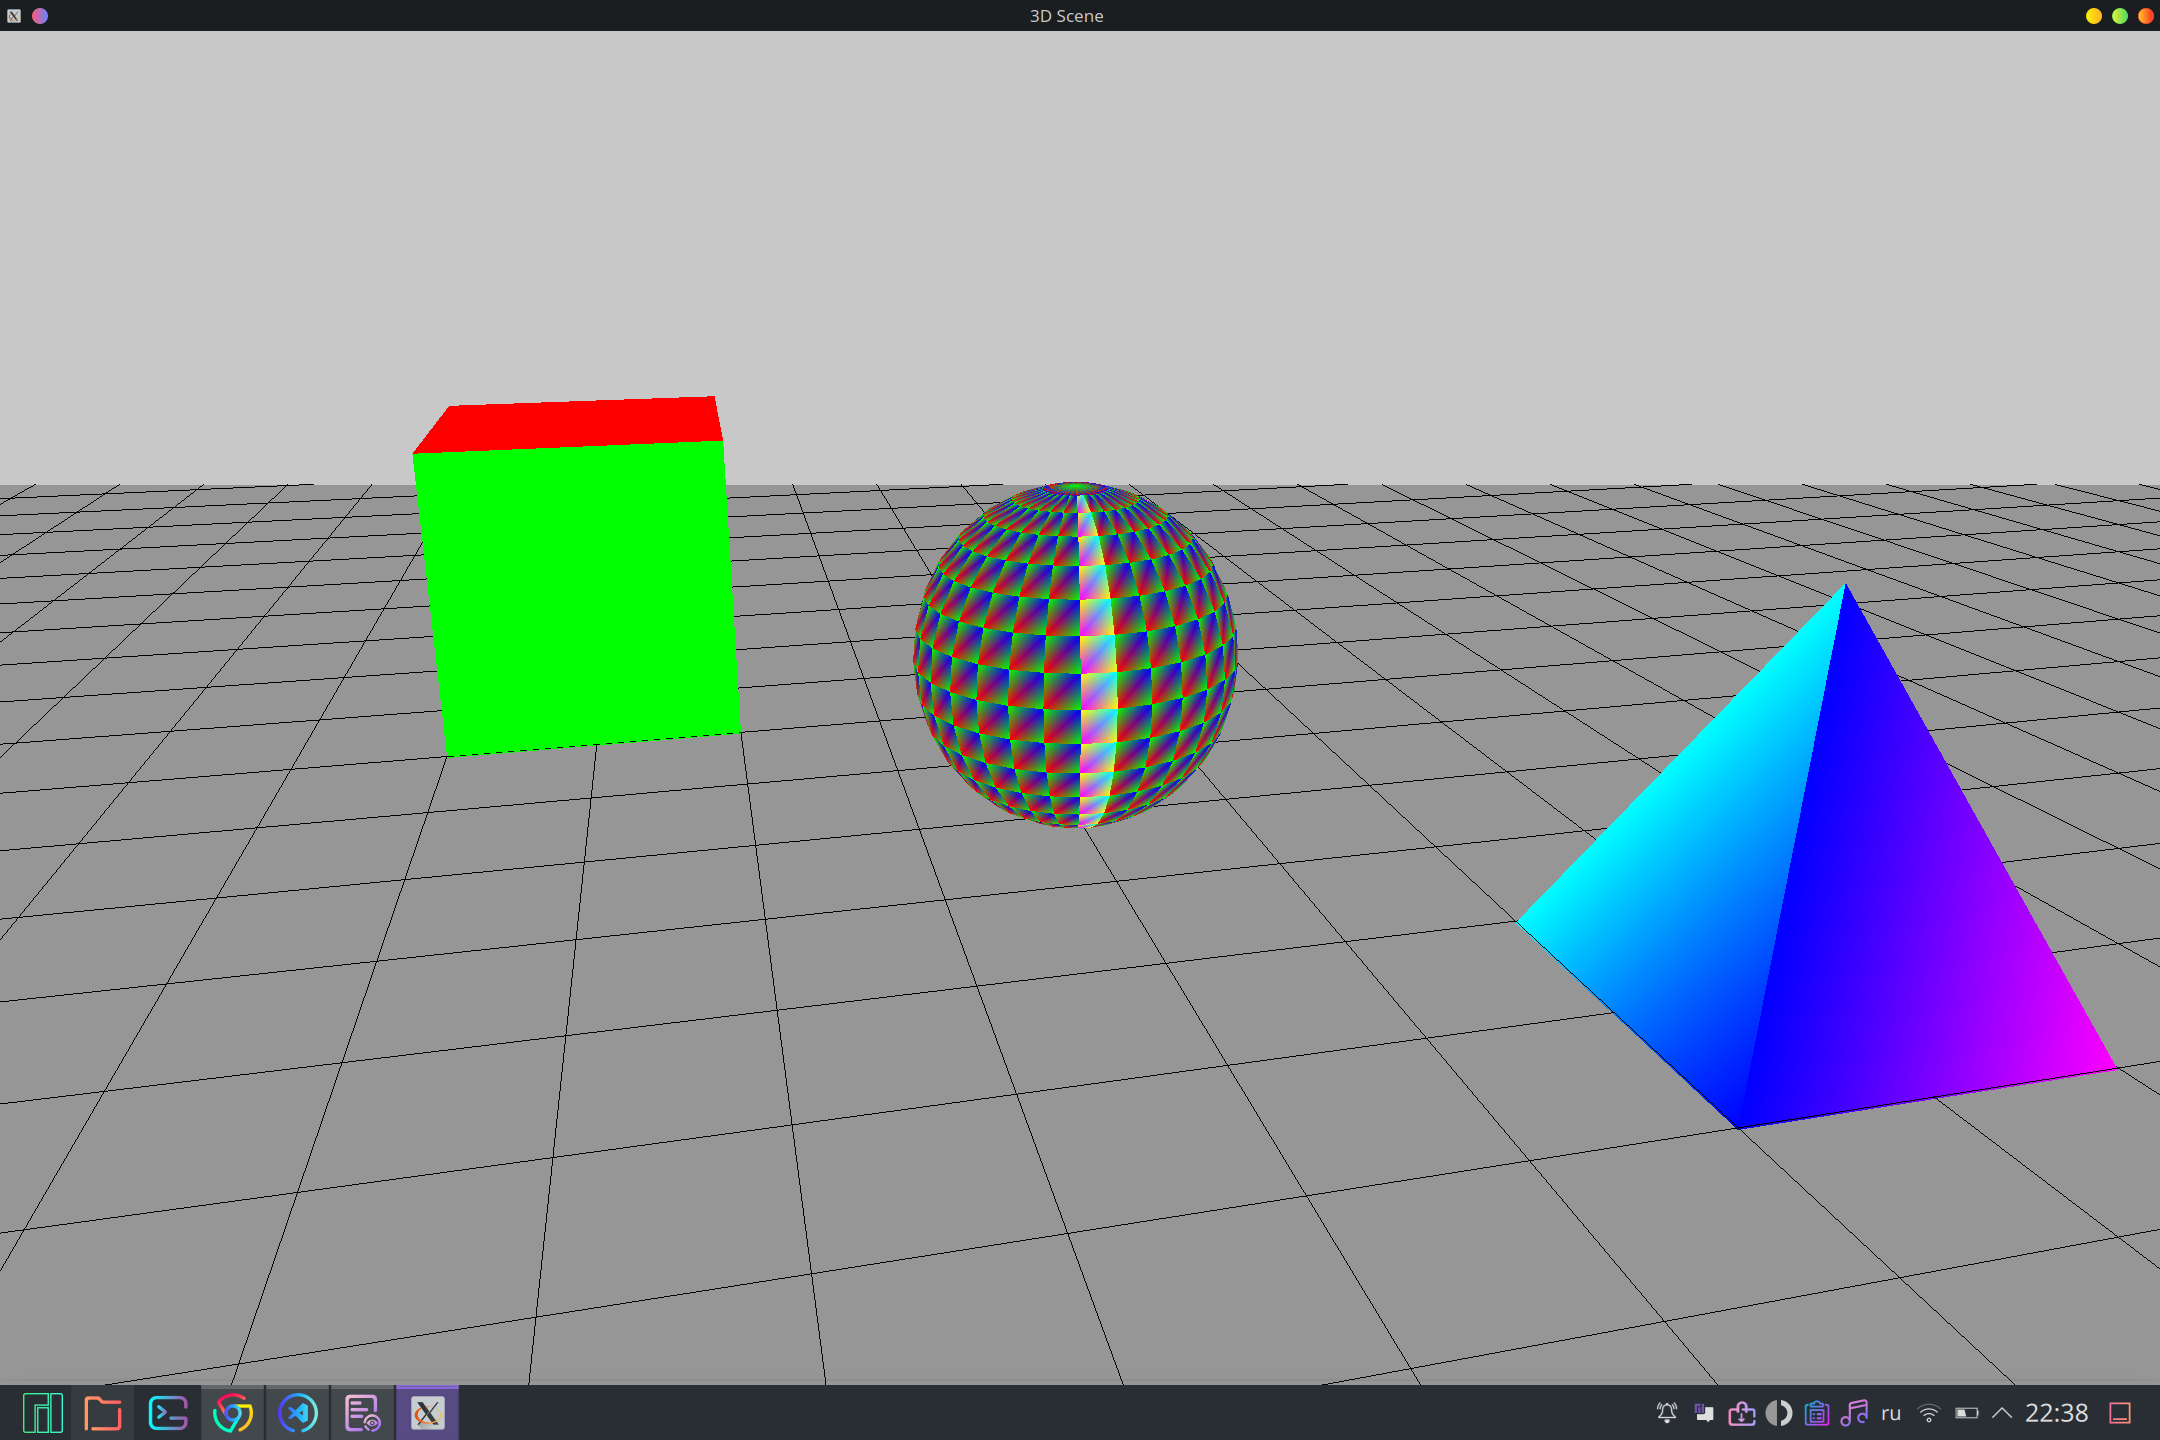
\includegraphics[width=15cm]{demo.png}

% \newpage
\subsection*{Выводы}

В процессе выполнения лабораторной работы я изучил основы работы с 3D-графикой
и библиотекой OpenGL. Я получил навыки работы с камерой в компьютерной графике, а также
научился настраивать взаимодействие пользователя с программой с помощью клавиш и мыши.

\end{document}